\documentclass[a4paper, 12pt]{article}
\usepackage[english]{babel} % or \usepackage[vietnamese]{babel}
\usepackage[utf8x]{inputenc}
\usepackage{amsmath, graphicx, tikz}
\usetikzlibrary{calc}
\usepackage[utf8]{vietnam}
\usepackage{enumerate}
\usepackage{scrextend}
\usepackage{amsmath}
\usepackage{amsfonts}
\usepackage{amssymb}
\usepackage{graphicx}
\usepackage{subfigure}
\usepackage{wrapfig}
%\usepackage{mathptmx}

\begin{document}

\begin{titlepage}
	
\begin{tikzpicture}[remember picture,overlay,inner sep=0,outer sep=0]
\draw[blue!70!black,line width=4pt] ([xshift=-1.5cm,yshift=-2cm]current page.north east) coordinate (A)--([xshift=1.5cm,yshift=-2cm]current page.north west) coordinate(B)--([xshift=1.5cm,yshift=2cm]current page.south west) coordinate (C)--([xshift=-1.5cm,yshift=2cm]current page.south east) coordinate(D)--cycle;

\draw ([yshift=0.5cm,xshift=-0.5cm]A)-- ([yshift=0.5cm,xshift=0.5cm]B)--
([yshift=-0.5cm,xshift=0.5cm]B) --([yshift=-0.5cm,xshift=-0.5cm]B)--([yshift=0.5cm,xshift=-0.5cm]C)--([yshift=0.5cm,xshift=0.5cm]C)--([yshift=-0.5cm,xshift=0.5cm]C)-- ([yshift=-0.5cm,xshift=-0.5cm]D)--([yshift=0.5cm,xshift=-0.5cm]D)--([yshift=0.5cm,xshift=0.5cm]D)--([yshift=-0.5cm,xshift=0.5cm]A)--([yshift=-0.5cm,xshift=-0.5cm]A)--([yshift=0.5cm,xshift=-0.5cm]A);

\draw ([yshift=-0.3cm,xshift=0.3cm]A)-- ([yshift=-0.3cm,xshift=-0.3cm]B)--
([yshift=0.3cm,xshift=-0.3cm]B) --([yshift=0.3cm,xshift=0.3cm]B)--([yshift=-0.3cm,xshift=0.3cm]C)--([yshift=-0.3cm,xshift=-0.3cm]C)--([yshift=0.3cm,xshift=-0.3cm]C)-- ([yshift=0.3cm,xshift=0.3cm]D)--([yshift=-0.3cm,xshift=0.3cm]D)--([yshift=-0.3cm,xshift=-0.3cm]D)--([yshift=0.3cm,xshift=-0.3cm]A)--([yshift=0.3cm,xshift=0.3cm]A)--([yshift=-0.3cm,xshift=0.3cm]A);

\end{tikzpicture}

\newcommand{\HRule}{\rule{\linewidth}{0.5mm}} % Defines a new command for the horizontal lines, change thickness here

\centering % Center everything on the page
 
%	HEADING SECTIONS
\textsc{\LARGE ĐẠI HỌC BÁCH KHOA TP. HCM}\\[1cm] % Name of your university/college
\textsc{\Large KHOA ĐIỆN ĐIỆN TỬ}\\[0.5cm] % Major heading such as course name
\textsc{\large BỘ MÔN TỰ ĐỘNG}\\[0.5cm] % Minor heading such as course title

%	TITLE SECTION
\HRule \\[0.4cm]
{ \huge \bfseries ĐỀ CƯƠNG TỐT NGHIỆP }\\[0.4cm] % Title of your document
\HRule \\[1cm]
 
%	AUTHOR SECTION
\begin{minipage}{0.4\textwidth}
\begin{flushleft} \large
\emph{Sinh viên:}\\
\textsc{Tạ Minh Đức} \\% Your name
\textsc{MSSV: 1510812}\\
\textsc{Huỳnh Nhật Tú} \\% Your name
\textsc{MSSV:  1513922}
 
\end{flushleft}
\end{minipage}
~
\begin{minipage}{0.4\textwidth}
\begin{flushright} \large
\emph{GVHD:} \\
\textsc{Thầy Nguyễn Vĩnh Hảo} % Supervisor's Name
\end{flushright}
\end{minipage}\\[1cm]

% If you don't want a supervisor, uncomment the two lines below and remove the section above
%\Large \emph{Author:}\\
%Vu \textsc{Hong Quan}\\[3cm] % Your name

%	LOGO SECTION

\includegraphics[scale=0.25]{images/LogoBK.jpg}\\[1cm] % Include a department/university logo - this will require the graphicx package

%	DATE SECTION
{\large \today}\\[0cm] % Date, change the \today to a set date if you want to be precise

\vfill % Fill the rest of the page with whitespace
\end{titlepage}

\tableofcontents
\changefontsizes{13pt}
% Tóm tắt nội dung
\newpage
\begin{abstract}
Mục tiêu đề tài là tìm hiểu và thực hiện điều khiển mô hình xe không người lái thông qua thiết bị định vị NEO - M8P, ứng dụng thuật toán điều khiển Stanley trong tính toán góc lái cho đối tượng và chương trình giám sát, điều khiển từ xa thông qua thiết bị thu phát sóng RF.\\
\indent
Đối tượng được thiết kế dựa trên mô hình Ackerman với 2 bánh được điều khiển độc lập và 1 bánh đa hướng. Đối tượng được xác định vị trí thông qua mạch Rover - Một trong hai mạch định vị GPS của NEO - M8P, mạch điều khiển cho toàn bộ đối tượng được sử dụng là Board STM32F411 Discovery cùng với các mạch được thiết kế để sử dụng trong quá trình điều khiển.\\
\indent
Một chương trình viết cho đối tượng được thiết kế để có thể giám sát, điều khiển từ xa, thu thập dữ liệu và các thao tác khác như điều khiển bằng tay từ xa, điều khiển tự động dựa trên thuật toán điều khiển hướng lái Stanley. Chương trình được viết trên C\# winform control.\\
\indent
Ứng dụng của Fuzzy trong điều khiển góc. Một bộ fuzzy PI được thiết kế để điều khiển góc cho đối tượng, bảng luật dựa trên kinh nghiệm và đặc tính của mô hình trong quá trình thử nghiệm mà lựa chọn thông số sao cho đối tượng đạt được độ chính xác theo yêu cầu.\\
\indent
Đối tượng là sản phẩm để thử nghiệm độ chính xác của thuật toán điều khiển, ứng dụng của nó trong việc tự động hóa các phương tiện sản suất di chuyển trong một không gian mà không cần đến người điều khiển.\\
\end{abstract}

% Phần 1 phần cứng
\newpage
\section{Phần cứng}

\newpage
\section{Phần mềm}
\subsection{Sơ đồ khối}
\subsubsection{Sơ đồ khối tổng}
\hspace{0.5cm}
Bài toán đặt ra là điều khiển mô hình theo tập dữ liệu tọa độ đã được thu thập trước (Tọa độ về đường đi lấy được thông qua GPS và được lưu về máy sử dụng cho việc điều khiển). Thuật toán Stanley với ngõ vào là tập dữ liệu về tọa độ x,y và góc hiện tại của mô hình để so với tọa độ đường đi rồi tính ra góc lái điều khiển mô hình về vị trí tọa độ gần nhất. Vì thế cần thiết kế một bộ điều khiển góc để mô hình có thể điều hướng theo góc một góc đặt được tính ra từ thuật toán Stanley trước đó. Sử dụng bộ điều khiển PI mờ với mục đích điều khiển góc sao cho sai số xác lập bằng 0 và đáp ứng ổn định, các thông số của bộ điều khiển PI được xác định dựa trên kinh nghiệm thực tế trong quá trình thử nghiệm mà thay đổi cho phù hợp. \\\indent
Từ đó suy ra sơ đồ khối tổng cho toàn bộ hệ thống như sau:\\\newpage
\begin{center}
	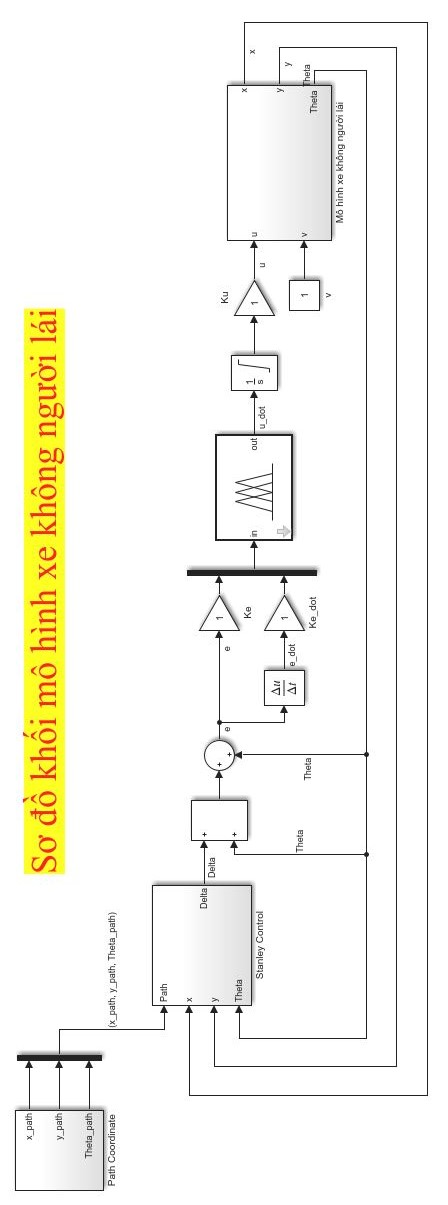
\includegraphics[width=340px,height=530px]{images/SoDoKhoiTong_Ngang}\\
	Hình 2.1. Sơ đồ khối của xe mô hình không người lái
\end{center}

\newpage
\subsubsection{Mô hình xe không người lái}
\hspace{0.5cm}
Đối tượng điều khiển là mô hình xe không người lái, được thiết kế với 2 động cơ, 1 bánh đa hướng, bộ xử lí trung tâm là Board STM32F411 Discovery, mạch NEO - M8P rover xác định vị trí, mạch thu phát RF truyền nhân thông tin giữa 2 mạch GPS và giữa mô hình với máy tính giám sát và điều khiển hoạt động.\\\indent
2 động cơ điều khiển bằng bộ điều khiển PID. Bằng cách thay đổi tốc độ giữa 2 động cơ sẽ có thể điều khiển được hướng của mô hình, vì thế vận tốc đặt là kết quả của vận tốc đặt cố định trừ cho tốc độ được tính từ bộ điều khiển PI mờ.\\
\subsubsection{Bộ điều khiển PI mờ}
\hspace{0.5cm}
Ưu điểm của bộ điều khiển PI mờ là đạt được sai số xác lập bằng 0, được sử dụng trong hệ thống không có khâu tích phân tuy nhiên đáp ứng chậm. Ứng dụng bộ điều khiển PI mờ trong việc điều khiển góc quay cho mô hình xe không người lái.\\\indent
Các bước thiết kế một bộ điều khiển PI mờ:\\
\begin{enumerate}
	\item Sơ đồ khối hệ thống:\\
	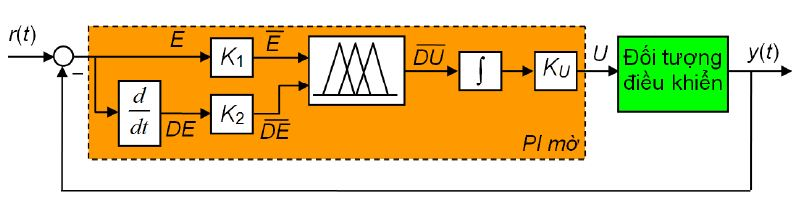
\includegraphics[width=400px,height=160px]{images/BDKPI}\\
	\begin{center}
		Hình 2.2. Sơ đồ khối bộ điều khiển PI mờ\\
	\end{center}
	\newpage
	- Xác định tầm giá trị:
	\begin{enumerate}
		\item[+] Biến vào: Sai số $e$ và vi phân sai số $\dot{e}$
		\item[+] Biến ra: Vi phân của tín hiệu điều khiển $\dot{u}$
	\end{enumerate}
	\item Chuẩn hóa giá trị biến vào và biến ra trong miền [-1,1]\\
	\begin{enumerate}
		\item[-] Chuẩn hóa giá trị sai số $e$\\\indent
		$ e = \theta_{d} - \theta $ với $ \theta_{d}:$ Góc đặt được tính từ khối Stanley Control; $\theta:$ Góc ngõ ra của đối tượng.\\\indent
		$\bullet$ $-\pi \le \theta_{d} \le \pi$ và $-\pi \le -\theta \le \pi$ nên $-2\pi \le e = \theta_{d} - \theta \le 2\pi$\\\indent
		$\bullet$ Chọn $K_{1} = \frac{1}{2\pi}$
		\item[-] Chuẩn hóa giá trị vi phân sai số $\dot{e}$\\
		$\dot{e} = \frac{\triangle e}{\triangle t}$ là tốc độ thay đổi của sai số. Chọn miền giá trị cho $ \dot{e} $: $ -\frac{\pi}{4} \le \dot{e} \le \frac{\pi}{4} $. Chọn $K_{2} = \frac{4}{\pi}$.
		\item[-] Chuẩn hóa giá trị vi phân của tín hiệu điều khiển $\dot{u}$//
		$\dot{u} = \frac{\triangle u}{\triangle t}$ là tốc độ thay đổi của tín hiệu điều khiển. Chọn miền giá trị cho $\dot{u}$: $-0.3 \le \dot{u} \le 0.3 (\frac{\%}{s})$. Chọn $K_{u} = 1$.
	\end{enumerate}
	\item Định nghĩa giá trị ngôn ngữ cho biến vào và biến ra; định lượng các giá trị ngôn ngữ bằng tập mờ\\
	Ngõ vào bộ điều khiển PI mờ có 2 ngõ vào là $e$ và $\dot{e}$:\\
	- Chọn 5 giá trị ngôn ngữ cho biến $e$: NB, NS, ZE, PS, PB\\
	- Chọn 3 giá trị ngôn ngữ cho biến $\dot{e}$: NE, ZE, PO\\
	Ngõ ra bộ điều khiển PI mờ có 1 ngõ ra là $\dot{u}$:\\
	- Chọn 7 giá trị ngôn ngữ cho biến $\dot{u}$: NB, NM, NS, ZE, PS, PM, PB.\\
	Định lượng giá trị 2 biến ngôn ngữ trên bằng tập mờ như sau:\\\newpage
	\begin{center}
		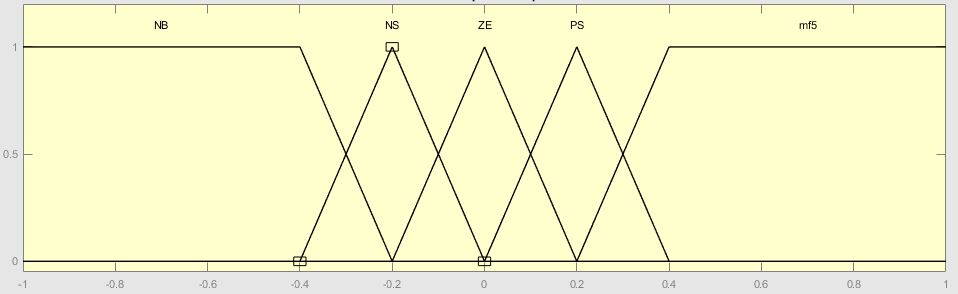
\includegraphics[width=350px,height=150px]{images/efigure}\\
		Hình 2.3. Tập mờ cho biến ngõ vào $e$\\
		\vspace{0.5cm}
		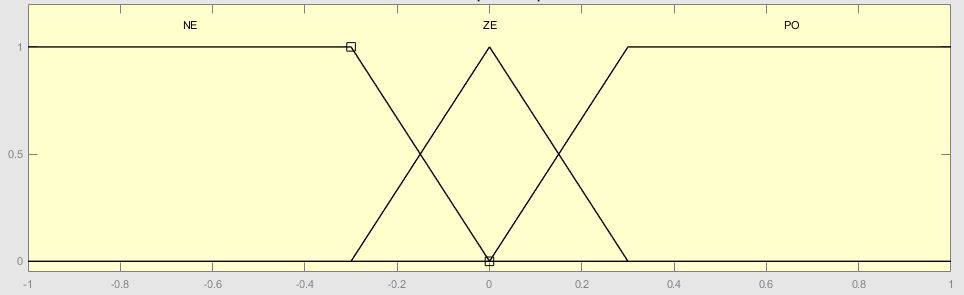
\includegraphics[width=350px,height=150px]{images/edotfigure}\\
		Hình 2.4. Tập mờ cho biến ngõ vào $\dot{e}$\\
		\vspace{0.5cm}
		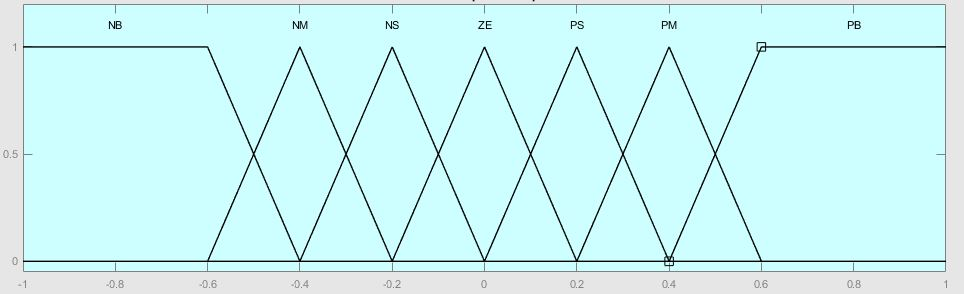
\includegraphics[width=350px,height=150px]{images/udotfigure}\\
		Hình 2.5. Tập mờ cho biến ngõ ra $\dot{u}$
	\end{center}
	\newpage
	Các giá trị cho biến ngôn ngữ được chọn dựa trên kinh nghiệm điều khiển thực tế mà có thể thay đổi sao cho hệ thống đạt được đáp ứng theo yêu cầu người điều khiển.
	\item Xây dựng bảng luật quy tắc mờ.\\
	Xây dựng bảng luật với 15 luật từ 2 biến ngõ vào cho 1 biến ngõ ra. Biểu diễn mô hình như hình vẽ, sự thay đổi góc của mô hình xảy ra nhờ việc thay đổi tốc độ một trong hai động cơ trái và phải. Giá trị thay đổi dựa trên phần trăm nhân với vận tốc đặt hiện tại của mô hình. Ví dụ khi rẽ phải thì động cơ bên phải sẽ lấy giá trị đặt nhân với $(1-u)$ và giữ nguyên giá trị đặt động cơ bên trái thì mô hình sẽ rẽ sang phải, tùy theo giá trị phần trăm tín hiệu điều khiển tính được từ bộ điều khiển PI mờ mà tốc độ thay đổi góc sẽ nhanh hay chậm. Và một cách tính tương tự cho bánh trái, vì thế mô hình có tính đối xứng.\\
	\begin{center}
		\includegraphics[width=300px,height=300px]{images/model}\\
		Hình 2.6. Mô hình xe không người lái sử dụng bộ điều khiển góc PI mờ
	\end{center}
	\begin{center}
		\begin{tabular}{|c|c|c|c|c|c|c|}
			\hline
			\multicolumn{2}{|c|}{$\bar{\dot{u}}$} & \multicolumn{5}{c}{$\bar{e}$} \vline \\\cline{3-7}
			\multicolumn{2}{|c|}{} \vline& NB & NS & ZE & PS & PB \\\hline
			& NE & NB & NM & NS & ZE & PS \\\cline{2-7}
			$\bar{\dot{e}}$ & ZE & NM &NS & ZE & PS & PM \\\cline{2-7}
			& PO & NS & ZE & PS & PM & PB \\\hline
		\end{tabular}\\\vspace{0.5cm} 
	Bảng 1: Bảng luật điều khiển góc PI mờ
	\end{center}
	Một số minh họa xác định luật điều khiển:\\
	\begin{center}
		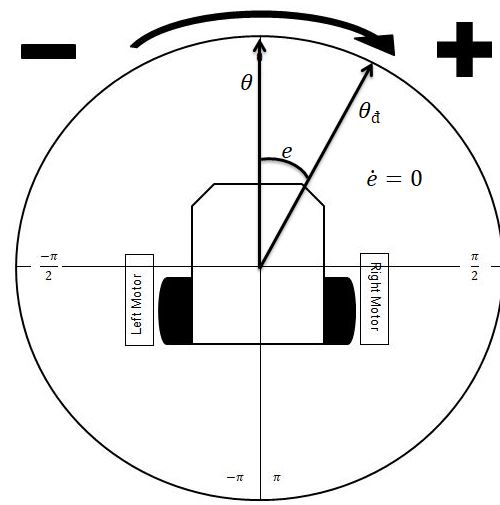
\includegraphics[width=150px,height=150px]{images/Case1}
	\end{center}
	$\bar{e} = PS$ và $\bar{\dot{e}} = ZE$. $\theta_{đ}$ lớn hơn $\theta$ một lượng PS, tốc độ thay đổi sai số bằng 0 nên phải tăng tốc độ thay đổi tín hiệu điều khiển một lượng PS.\\
	\begin{center}
		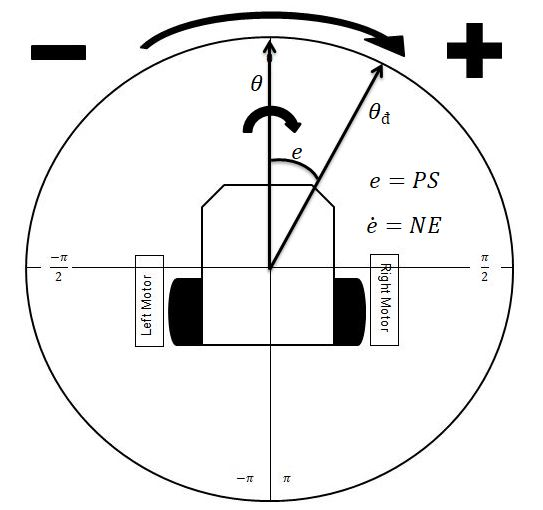
\includegraphics[width=150px,height=150px]{images/Case2}
	\end{center}
	$\bar{e} = PS$ và $\bar{\dot{e}} = NE$. $\theta_{đ}$ lớn hơn $\theta$ một lượng PS, tốc độ thay đổi sai số là âm ứng với $\theta$ đang có xu hướng quay cùng chiều kim đồng hồ về góc $\theta_{đ}$ nên ngõ ra không cần thay đổi, $\bar{\dot{u}}$ = ZE.\\
	\begin{center}
		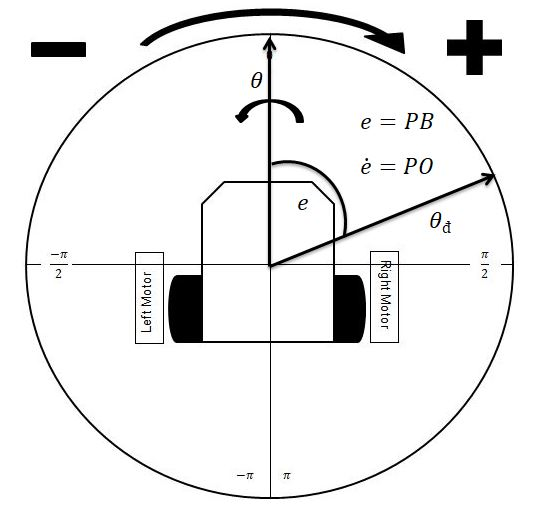
\includegraphics[width=150px,height=150px]{images/Case3}
	\end{center}
	$\bar{e} = PB$ và $\bar{\dot{e}} = PO$. $\theta_{đ}$ lớn hơn $\theta$ một lượng PB, tốc độ thay đổi sai số là dương ứng với $\theta$ đang có xu hướng quay ngược chiều kim đồng hồ và ngày càng ra xa khỏi $\theta_{đ}$ nên cần tăng một lượng PB có xu hướng cùng chiều kim đồng hồ.\\
	\begin{center}
		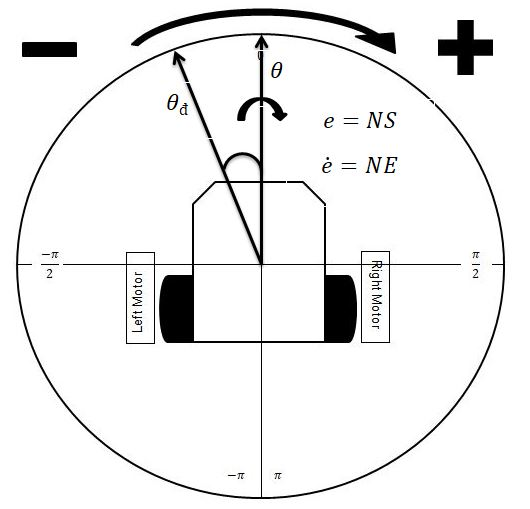
\includegraphics[width=150px,height=150px]{images/Case4}
	\end{center}
	$\bar{e} = NS$ và $\bar{\dot{e}} = NE$. $\theta_{đ}$ nhỏ hơn $\theta$ một lượng PB, tốc độ thay đổi sai số là âm ứng với $\theta$ đang có xu hướng quay cùng chiều kim đồng hồ và ra xa khỏi $\theta_{đ}$ nên cần tăng một lượng NM có xu hướng ngược chiều kim đồng hồ.\\
	\item Chọn phương pháp suy diễn Max-Min
	\item Chọn phương pháp giải mờ trung bình có trọng số
	\item Thử nghiệm trên mô hình và điều chỉnh thông số cho các biến vào và ra sao cho đặt được đáp ứng hệ thống mong muốn.
\end{enumerate}
\newpage
\subsubsection{Stanley control}
\hspace{0.5cm}
\begin{center}
	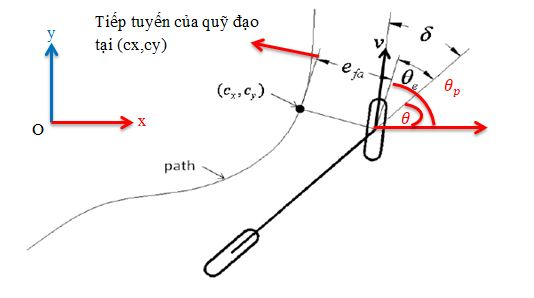
\includegraphics[width=350px,height=180px]{images/Stanley}\\
	Hình 2.7. Biểu diễn hình học cho phương pháp Stanley
\end{center}
\hspace{0.5cm}
Phương pháp Stanley là phương pháp tiếp cận cho ứng dụng Robot dò theo quỹ đạo cho trước được phát triển bởi nhóm nghiên cứu về phương tiện tự hành (UAV) của trường đại học Stanford (Mỹ) đã đoạt giải trong cuộc thi do DARPA (Defense Advanced Research Projects Agency ) tổ chức: The DARPA Grand Challenge. Phương pháp Stanley sử dụng phương trình hồi tiếp phi tuyến để tính toán góc quay của Robot dựa trên khoảng cách từ tâm Robot tới 1 điểm trên quỹ đạo và sai số góc giữa tiếp tuyến quỹ đạo tại điểm đang xét với phương dọc của Robot.\\\indent
Phương pháp Stanley sử dụng 2 điều kiện để tính toán ra góc quay của Robot. Điều kiện thứ nhất trong luật điều khiển Stanley là sai số giữa góc lệnh tiếp tuyến tại 1 điểm trên quỹ đạo đường – (cx,cy), gần với tâm của trục bánh trước nhất và góc lệnh của phương dọc xe so với trục x (được biểu diễn trên hình 1). Bằng cách cân bằng được giữa giá trị góc lệnh của xe so với sai số của giá trị điều kiện thứ nhất trong luật điều khiển của Stanley thì ta có thể giữ cho trục thân xe song song với tiếp tuyến của quỹ đạo đường.\\
\begin{center}
	$\theta_{e} = \theta_{p} - \theta$ (1)
\end{center}
\begin{enumerate}
	\item[-] Với $\theta_{e}$ là sai số góc giữa tiếp tuyến tại 1 điểm được xét trên quỹ đạo đường với góc của trục thân xe so với trục x.
	\item[-] $\theta_{p}$ là góc lệnh của tiếp tuyến quỹ đạo tại (cx,cy) với trục x.
	\item[-] $\theta$ là góc lệnh của trục Robot với trục x.
\end{enumerate}
\hspace{0.5cm}
Từ phương trình (1) có thể thấy nếu góc điều khiển $\delta$ như trên hình 1 mà bằng với $\theta_{e}$ thì xe và tiếp tuyến quỹ đạo song song nhau, nhưng chưa bám được quỹ đạo khi $e_{fa}$ khác 0. Trường hợp như hình 1 là $e_{fa}$ khác 0 thì điều kiện thứ 2 trong luật điều khiển Stanley sẽ điều chỉnh góc quay sao cho xe và tiếp tuyến quỹ đạo mong muốn giao nhau tại (cx,cy) tại kv(t) từ trục bánh trước, tùy thuộc vào v(t) của xe để luật điều khiển có thể thể bám tốt. Ta có luật điều khiển Stanley hoàn chỉnh:\\
\begin{center}
	$\delta(t) = \theta_{e}(t) + arctan(\frac{ke_{fa}(t)}{v_{x}(t)})$ (2)
\end{center}
- Với k là gain để hiệu chỉnh luật điều khiển.\\
\indent
Sơ đồ khối sử dụng bộ xử lí Stanley để tính ra góc lệch cần điều khiển cho mô hình xe không người lái:
\begin{center}
	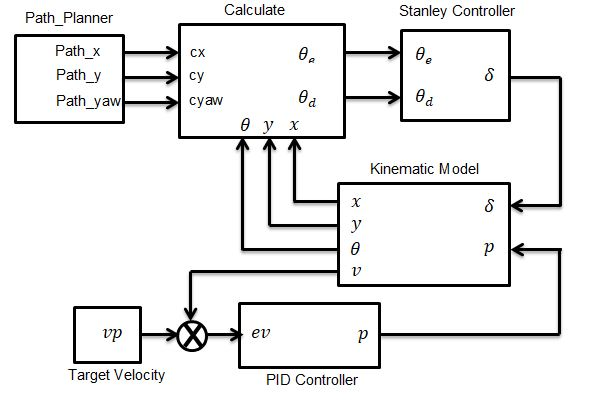
\includegraphics[width=350px,height=280px]{images/SoDoKhoiStanley}\\
	Hình 2.8. Sơ đồ khối tính toán góc lệch cần điều khiển cho mô hình sử dụng phương pháp Stanley
\end{center}
\hspace{0.5cm}
Sơ đồ khối ở trên tuần tự ta có các khối:\\
\begin{enumerate}
	\item[-] Khối Path Planner là khối khởi tạo 3 tập giá trị của quỹ đạo mong muốn bao gồm giá trị tọa độ x,y và giá trị góc lệch của tiếp tuyến quỹ đạo với trục x. 
	\item[-] Khối Calculate là khối tính toán khoảng cách ngắn nhất từ tâm trục bánh trước tới 1 điểm trên quỹ đạo từ đó tính được góc lệch $\theta_{d}$  là điều kiện thứ 2 trong luật điều khiển Stanley.
	\item[-] Khối Stanley Controller lấy 2 giá trị ngõ ra tính được từ khối Calculate để suy ra góc điều khiển $\delta$
	\item[-] Khối PID Controller điều khiển vận tốc đối tượng theo vận tốc đặt mong muốn.
	\item[-] Khối Kinematic Model là mô hình thực tế của đối tượng xe không người lái.
\end{enumerate}
\subsection{Giải thuật điều khiển}
\hspace{0.5cm}
Để thuận tiện trong việc điều khiển, cần thiết kế giao diện điều khiển cũng như giám sát trong suốt quá trình vận hành nhằm mục đích quan sát và đánh giá hoạt động của hệ thống. Giao diện chính điều khiển được thiết kế trên máy tính bằng ứng dụng Window Form Control $C\#$.\\
\indent
Giao tiếp giữa mô hình và máy tính thông qua 2 thiết bị truyền nhận sóng RF đã miêu tả ở phần cứng. Thông tin được truyền theo chuẩn USART, format được qui định cụ thể cho mỗi tác vụ.\\
\indent
Có 2 chế độ điều khiển là Manual (Chỉnh tay) và Auto (Tự động). Ở chế độ Manual, mô hình được điều khiển bằng tay, còn ở chế độ Auto mô hình tự động vận hành bằng thuật toán đã mô tả ở phần trước.
\subsubsection{Giao diện điều khiển}
Giao diện được viết bằng ngôn ngữ $C\#$. Giao diện chính chia thành các User Control để dễ dàng quản lí và thiết kế. Có 3 giao diện nhỏ khác nhau: Setting, Manual và Auto.
\hspace{0.5cm}
\begin{center}
	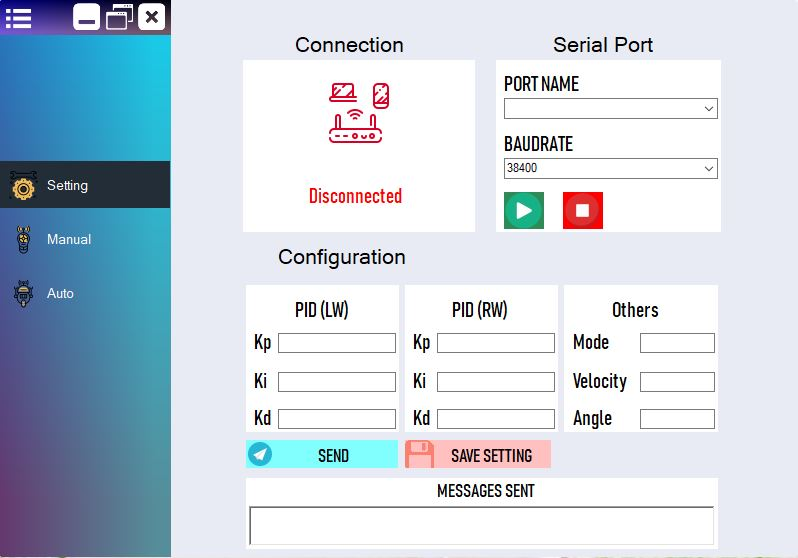
\includegraphics[width=350px,height=260px]{images/InterfaceSetting}\\
	Hình 2.9. Giao diện điều khiển Settings\\\vspace{0.5cm}
	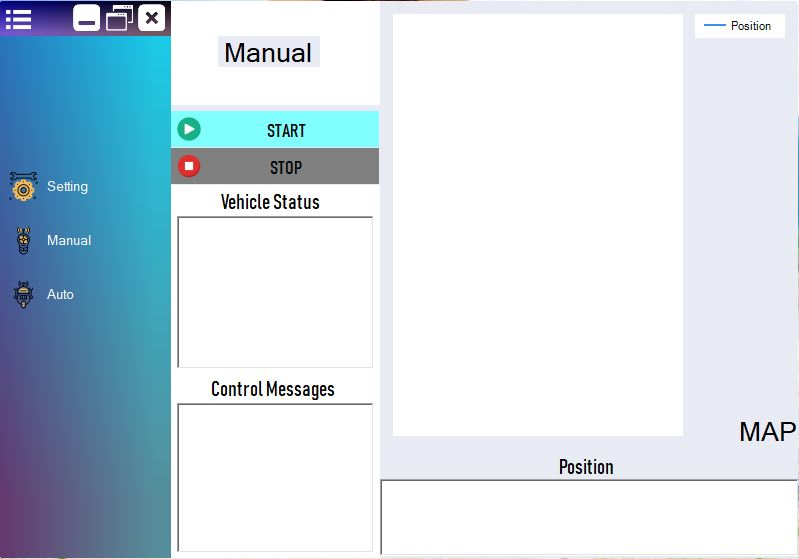
\includegraphics[width=350px,height=260px]{images/InterfaceManual}\\
	Hình 2.10. Giao diện điều khiển Auto/Manual
\end{center}
\newpage
\subsection{Thử nghiệm mô hình}
\hspace{0.5cm}
Thử nghiệm hệ thống sau khi đã hoàn tất thiết kế, cố định các mạch xử lí và module điều khiển vào mô hình. Sau đó cấp nguồn vào hệ thống, sử dụng phần mềm Serial Port Hercules để thử nghiệm gửi thông tin diều khiển xuống mô hình thông qua mạch giao tiếp USART. Kiếm tra tham số, các giá trị biến thay đổi, sử dụng phần mềm STM Studio để quan sát và đánh giá hoạt động của mô hình sau khi viết chương trình điều khiển cho Board STM32F411 Discovery.\\\indent
Các bước thực hiện kiếm tra chương trình thiết kế:\\
\begin{enumerate}
	\item Kết nối mô hình với chương trình Serial Port Hercules trên máy tính
	
	\item Khởi tạo các biến cần kiếm tra trong phần mềm STM Studio
	
	\item Gửi thông tin điều khiển xuống mô hình thông qua Serial Port để xem đáp ứng hệ thống
	
	\item Thu nhận kết quả điều khiển
	
\end{enumerate}
\newpage
\subsection{Kết quả điều khiển hệ thống thông qua giao diện}
\hspace{0.5cm}
Sau khi kiếm tra hoạt động bằng STM Studio và Serial Port, tiếp theo là dùng giao diện điều khiển vừa thiết kế để tiếp tục việc kiểm tra hoạt động của giao diện.\\\indent
Các bước kiếm tra chất lượng của giao diện vừa thiết kế:\\
\begin{enumerate}
	\item Mở giao diện và khởi tạo kết nối Serial Port với mô hình
	
	\item Gửi thông tin điều khiển từ giao diện xuống mô hình
	
	\item Thu nhận kết quả điều khiển
\end{enumerate}
\end{document}






